\section{Воздействие радиоактивного излучения на электронные системы}

Проникающая радиация и радиоактивное заражение (ионизирующие излучения) могут изменять качество и свойства некоторых материалов, используемых в электронных системах, что приводит к сбоям и даже отказам в работе этих систем.

Особенно подвержены воздействию ионизирующих излучений полупроводниковые, газоразрядные, вакуумные приборы, некоторые типы конденсаторов и резисторов, органические материалы. Из неорганических материалов наиболее подвержены воздействию ионизирующих излучений оптические стекла, которые под действием излучений могут существенно увеличивать оптическую плотность~\cite{econ1}.

Современные интегральные микросхемы находят все более широкое применение в радиоэлектронной аппаратуре различного рода технических объектов, работающих в условиях воздействия проникающей радиации. Эти условия могут возникать при попадании объекта в зону действия источников ионизирующего излучения техногенного происхождения или при расположении вблизи ядерных силовых и энергетических установок, а на аппаратуру космических объектов воздействуют ионизирующие излучения космического пространства и радиационных поясов Земли. При этом радиоэлектронная аппаратура (РЭА) может подвергаться воздействию следующих уровней радиации:

\begin{itemize}
    \item от ядерного взрыва --- потоку нейтронов до 1015 на $\textrm{см}^2$ и гамма-квантов с экспозиционной дозой до 106 Рад при мощности дозы до 1013 Р/с;
    \item вблизи ядерных реакторов --- потоку нейтронов 1012--1015 и дозе гамма-квантов до 107 Рад~\cite{econ1}.
\end{itemize}

Высокая стоимость радиоэлектронных систем обуславливает особо жесткие требования к безотказности элементной базы радиоэлектронной аппаратуры и, в первую очередь, к микросхемам различного функционального назначения. Действительно, отказ одной микросхемы в условиях воздействия вышеперечисленных дестабилизирующих факторов может повлечь за собой выход из строя всего сложного и дорогостоящего объекта, причем последствия подобного отказа не всегда предсказуемы. Поэтому задача гарантированного обеспечения радиационной стойкости интегральных микросхем и аппаратуры на их основе является исключительно актуальной.

\section{Оценка устойчивости проектируемой системы к радиоактивному излучению}

Радиационная стойкость --- способность материалов сохранять исходный химический состав, структуру и свойства в процессе и (или) после воздействия ионизирующих излучений (ИИ).

Радиационная стойкость существенно зависит от вида радиации, величины и мощности поглощенной дозы, режима облучения (непрерывное или импульсное, кратковременное или длительное), условий эксплуатации материала (температура, высокое давление, механические нагрузки, магнитное или электрическое поле), размеров оfбразца материала и других факторов. На практике изменение свойств материала сопоставляется с величиной, характеризующей величину воздействующего излучения, например с потоком (флюенсом) нейтронов или поглощенной дозой ИИ. Количественной характеристикой часто служит также максимальное (предельное) значение поглощенной дозы и (или) мощности поглощенной дозы излучения, при котором материал становится непригодным для конкретных условий применения или до заданной степени меняет значение характерного параметра. Обычно проводят ускоренные радиационные испытания в лабораторных условиях, имитирующих эксплуатационные.

Возникающие в результате радиационно-индукционных процессов ионы и свободные электроны могут участвовать в сложных цепях физико-химических превращений (образование новых молекул и свободных радикалов, изменение кристаллической структуры и др.), совокупно приводящих к изменению механических, электрических, материальных, оптических и других свойств материалов. Изменения в материалах могут быть обратимыми или необратимыми и произойти как непосредственно вслед за радиационным воздействием, так и в течение длительного времени после акта облучения.

Радиационная стойкость неорганических веществ зависит от кристаллической структуры и типа химической связи. Наиболее стойки ионные кристаллы. Плотные структуры с высокой симметрией наиболее устойчивы к воздействию излучений. Для стекол характерно изменение прозрачности и появление окраски; возможна кристаллизация. Силикаты начинают изменять свойства после облучения флюенсом нейтронов ~1019 $\textrm{см}^2$. В результате облучения происходят: анизотропное расширение кристалла, аморфизация его структуры, уменьшение плотности, упругости, теплопроводности и других свойств. Оксиды при облучении нейтронами меняют свои свойства аналогично силикатам, но в меньшей степени. В свойствах бетонов существующие изменения отсутствуют при облучении флюенсом нейтронов до $3 \cdot 1019 \textrm{см}^2$.

Свойства металлов изменяются в зависимости от повреждений кристаллической решетки. Одиночные дефекты обычно упрочняют металл, но снижают его пластичность. Электрическое сопротивление металлов или сплавов возрастает за счет образования дефектов, хотя в сплавах возможно и уменьшение электрического сопротивления, если радиационное воздействие приводит к упорядочению структуры. В полупроводниках всегда имеется некоторая равновесная при определенной температуре концентрация точечных дефектов. Под действием облучения она увеличивается, что приводит к изменению электрических и оптических свойств полупроводников~\cite{econ2}.

Радиационная стойкость органических материалов принято определять величиной радиационно-химического выхода продуктов радиолиза, образующихся при поглощении 100 эВ энергии ИИ. Взаимодействие ИИ с орг. соед. сопровождается образованием промежуточных активных частиц, деструкцией, окислением, сшиванием, газообразованием, деполимеризацией (для полимеров) и т. д. Низкой радиационной стойкостью обладают вещества, содержащие связи С—F, С — Si, С—О. Наличие в молекуле двойных и сопряженных связей, ароматических колец и гетероциклов увеличивает радиационную стойкость. Наиболее значительные изменения структуры полимерных материалов под действием ИИ происходят при деструкции или сшивании молекул полимера.

Радиационная стойкость, в т. ч. полимеров, зависит и от количества растворенного в них О2 воздуха и скорости его поступления из окружающей среды; в его присутствии происходит радиационно-химическое окисление вещества. В результате этого существенно изменяются химическая и термическая стойкость веществ, предел прочности и модуль упругости, диэлектрическая проницаемость, электрическая прочность и электрическая проводимость.

Обратимые изменения в органических материалах обусловлены установлением стационарного равновесия между генерированием нестабильных продуктов радиолиза и их гибелью и зависят от мощности дозы. Так, электрическое сопротивление органических изоляционных материалов с увеличением мощности дозы падает на несколько порядков. При больших дозах снижение остаточного электрического сопротивления носит необратимый характер. У многих полимерных материалов, облученных дозами до 106 Гр, исходная электрическая проводимость меняется в несколько раз. При дозе 104 Гр необратимые изменения, как правило, незначительны. В органических полимерных материалах может возникать послерадиационное старение, которое обусловлено в основном химическими реакциями образовавшихся свободных радикалов с О2 воздуха. Радиационная стойкость полимерных диэлектриков ограничивается, как правило, их механическими свойствами, т. к. они становятся хрупкими и теряют способность нести механические нагрузки после доз, не вызывающих существенных изменений электрических св-в.

На рисунке~\ref{fig:table} представлены значения дозы облучения, вызывающие заметные (до 50\%) изменения свойств некоторых материалов.

\begin{figure}[ht]
    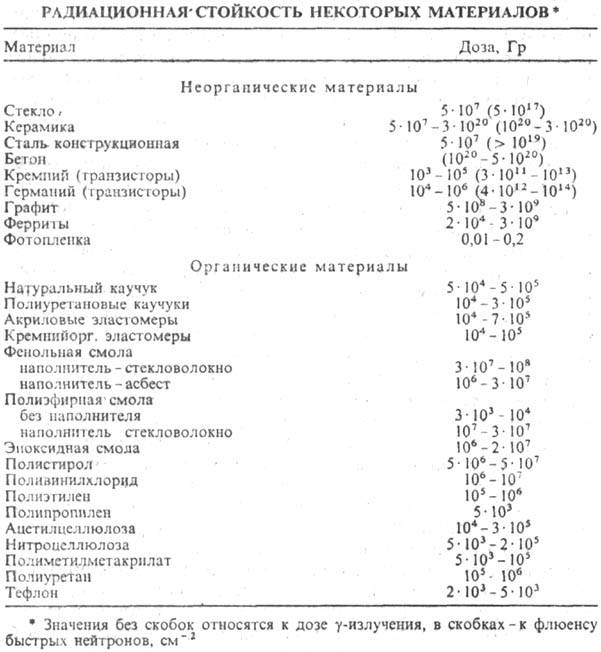
\includegraphics[width=.8\linewidth]{Figures/table.jpg}
    \caption{Заметные изменения свойств некоторых материалов}
    \label{fig:table}
\end{figure}

Для повышения радиационной стойкости обычно используют пассивную защиту (экранирование), физико-химические модификацию материала, радиационно-термическую обработку. Использование защитного экранирования снижает степень воздействия ИИ на материал. Таким путем в весьма широких пределах можно "повысить" стойкость любого материала. При физико-химической модификации в материал вводят добавки --- например, антиоксиданты, таким путем радиационная стойкость может быть повышена в 7-20 раз. Предварительная радиационно-термическая обработка-облучение и отжиг позволяет увеличить радиационную стойкость металлических материалов в 10-50 раз.

\bibliography{web,books}
